Agricultural technologies have been a source of innovation since the dawn of humanity. The quest for more efficient food
production has driven significant research, and above all, automation stands out as a paramount achievement in the
modern world. One of the tools used to improve the automation process is \gls{IoT}, a paradigm that refers to the interconnection
of physical devices in a diffused network in which each device collects valuable and localized information that is used to
improve efficiency, productivity, and decision making.\\
Many technologies implement the concepts described by \gls{IoT} using disparate approaches, furthermore, various
architectures describe the interaction between them. The most basic model proposes a stack composed of three layers:
\begin{itemize}
    \item a Perception layer, that collects data from sensors;
    \item a Network layer, that connects devices to falcilitate the exchange of information;
    \item an Application layer, that processes the data and makes it available.
\end{itemize}
The Network layer can be split further according to the \gls{ISO/OSI} model, in order to distinguish the purposes of the
communication protocols. Figure \ref{img: iso_osi} gives a representation of the stack and its components.
\begin{figure}[ht]
    \centering
    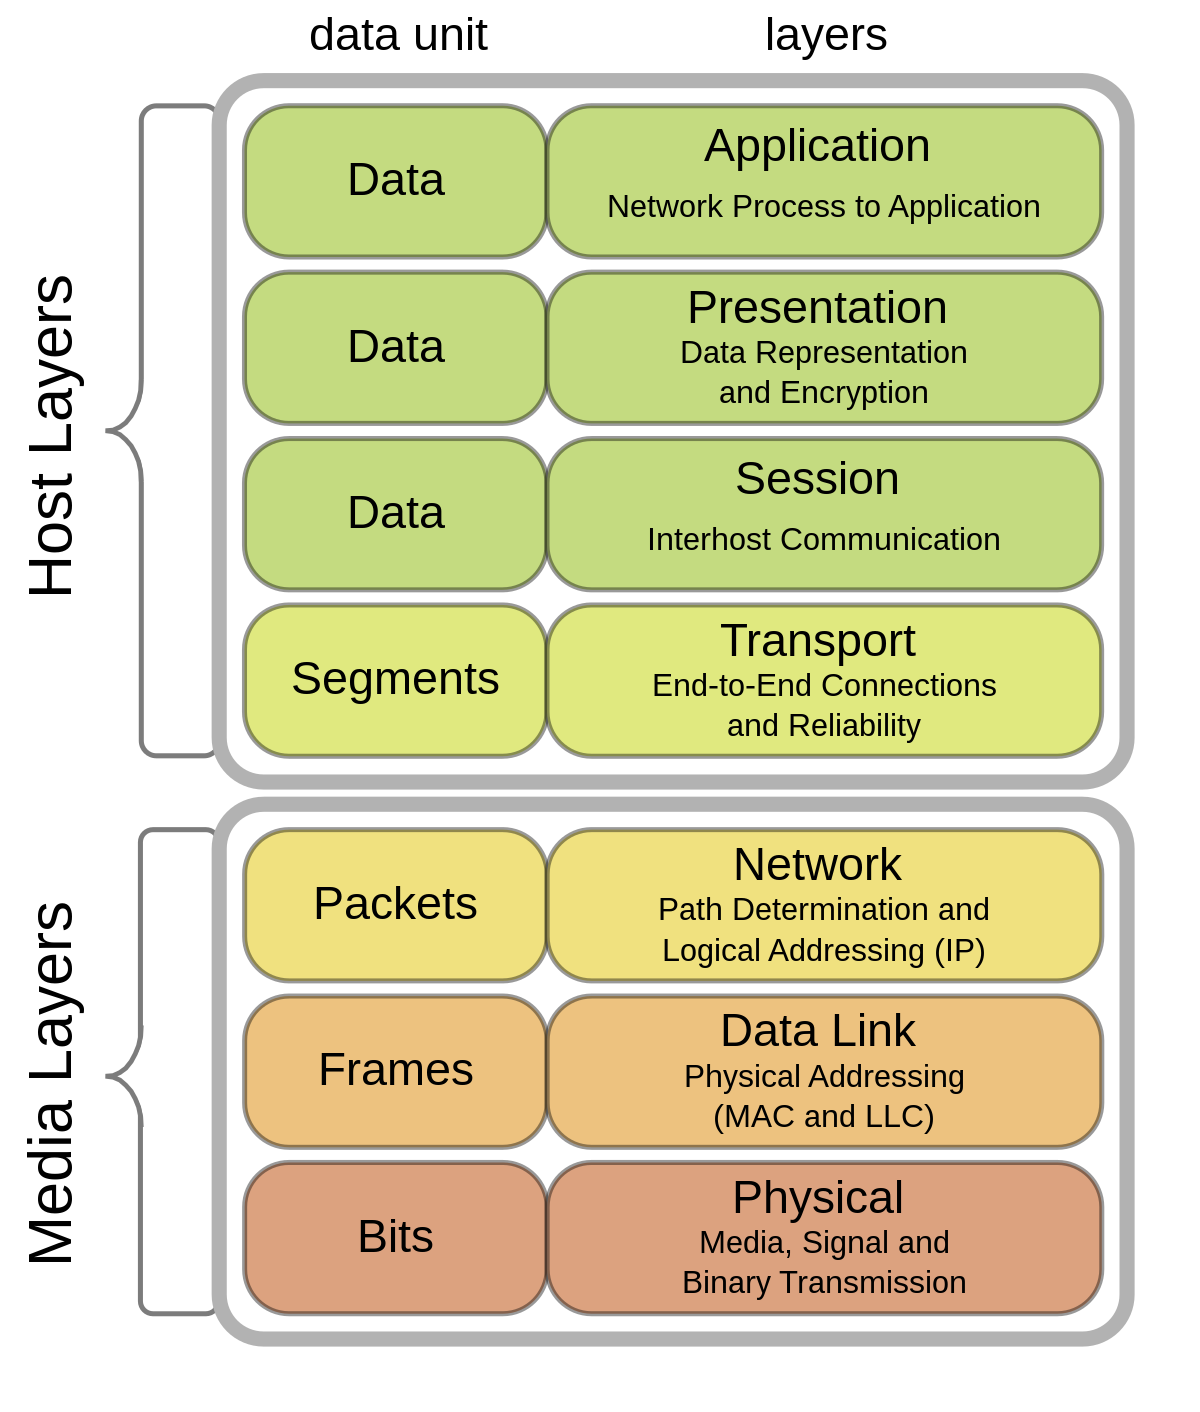
\includegraphics[width=0.5\linewidth]{images/iso_osi.png}
    \caption{ISO/OSI networking stack.}
    \label{img: iso_osi}
\end{figure}
The lowest layer of the stack is called physical layer, it takes care of electrical, mechanical and procedural
interfaces that directly concern the transmission medium. There resides LoRa, a protocol that has proven itself to be one
of the most fitting to construct \glspl{LPWAN} that follow the \gls{IoT} paradigm. This fact is validated by
extensive research, see \cite{lora_research_1} \cite{lora_research_2}, and by market analyses, in fact LoRa based
\gls{IoT} is estimated at USD 5.6 billion in 2023 and is projected at USD 25.5 billion by 2028 \cite{lora_marketshare}.
The areas of application of this technology are health care, logistics, transportation, smart homes, and many
others.\\
As stated above, the thesis will focus on applications in the field of agriculture, by presenting a \gls{MAC} layer
protocol called Bacco; it makes use of LoRa \gls{PHY} to construct \glspl{LPWAN} used for exchanging data collected by
localized sensors placed on-site. In order to do so, the thesis is organized as follows:
\begin{itemize}
    \item Chapter 1 provides an overview of the advantages and prerequisites of implementing \gls{IoT} in agriculture.
        Furthermore, it introduces Bacco and \gls{LoRaWAN}, the industry-standard \gls{MAC} protocol used for
        implementing LoRa-based \glspl{LPWAN};
    \item Chapter 2 describes the protocol and its specifics in depth;
    \item Chapter 3 discusses and compares the physical performance of Bacco and \gls{LoRaWAN} with calculations and
        laboratory tests.
\end{itemize}
